\documentclass[12pt, a4paper]{report}

% --- Essential Packages ---
\usepackage[utf8]{inputenc}
\usepackage[T1]{fontenc}
\usepackage{mathpazo} % Uses a beautiful, readable font (Palatino)
\usepackage{geometry}
\geometry{a4paper, margin=1.2in} % Comfortable margins
\usepackage{setspace}
\setstretch{1.2} % Slight line spacing for readability
\usepackage{amsmath}  % Required for \text{} inside equations
\usepackage{amssymb}  % Extra math symbols
\usepackage{booktabs} % Cleaner table rules
\usepackage{xcolor}
\usepackage{tikz}     % Required to draw the architecture diagrams
\usetikzlibrary{positioning, arrows.meta, calc, shapes.geometric, fit, backgrounds}

% --- Node palette for the graph architecture diagram ---
\definecolor{encblue}{HTML}{D6E4F7}   \definecolor{encline}{HTML}{2C5AA0}
\definecolor{fusteal}{HTML}{CCE9E2}   \definecolor{fusline}{HTML}{147A63}
\definecolor{retbrown}{HTML}{EADBC8}  \definecolor{retline}{HTML}{8A6132}
\definecolor{svcorange}{HTML}{FBE0C4} \definecolor{svcline}{HTML}{B5701A}
\definecolor{supviolet}{HTML}{E2DAF5} \definecolor{supline}{HTML}{5B45A8}
\definecolor{attgreen}{HTML}{DAECD0}  \definecolor{attline}{HTML}{4A7A2B}
\definecolor{gatered}{HTML}{F8D7D7}   \definecolor{gateline}{HTML}{B32B2B}
\definecolor{darkslate}{HTML}{D8DCE2} \definecolor{darkline}{HTML}{41505F}
\usepackage{titlesec}
\usepackage{hyperref} % hyperref should be loaded last

% --- Styling for Chapter Headings ---
\titleformat{\chapter}[display]
  {\normalfont\bfseries\Huge}
  {\hrulefill\vspace{2pt}\\ \chaptertitlename~\thechapter}
  {10pt}
  {\Huge}
  [\vspace{2pt}\hrulefill]

\hypersetup{
    colorlinks=true,
    linkcolor=blue,
    filecolor=magenta,
    urlcolor=cyan,
    pdftitle={Thesis: Agentic Multimodal RAG}
}

\begin{document}

% --- Custom Title Page ---
\begin{titlepage}
    \centering
    \vspace*{2cm}

    {\Huge \textbf{Agentic Multimodal RAG with Grounded Explanations for Complex Scientific Reasoning}\par}
    \vspace{2cm}

    \vfill
    {\large \today\par}
\end{titlepage}

% --- Abstract ---
\begin{abstract}
As the volume of scientific literature grows, researchers increasingly rely on AI-assisted literature review systems. However, current multimodal Retrieval-Augmented Generation (RAG) models operate on a passive, single-pass paradigm, leading to severe factual hallucinations on complex, multi-hop scientific queries. Furthermore, these systems act as ``black boxes,'' providing no verifiable visual grounding for their claims. In this thesis, we propose an Agentic Multimodal RAG framework that utilizes an iterative reasoning loop to dynamically fetch text, tables, and figures. By integrating an Evidence Sufficiency Gate before generation, a Faithfulness Gate after it, and a Grounded Explainability Module, our system generates precise spatial bounding boxes and retrieval execution logs. We outline a methodology to benchmark this framework on the SPIQA dataset, establishing a new standard for trust and verifiability in AI-assisted scientific document understanding.
\end{abstract}

% --- Table of Contents ---
\tableofcontents
\newpage

% --- Main Content ---
\chapter{Introduction}
\label{sec:introduction}

Researchers increasingly rely on AI-assisted literature review systems powered by Large Vision-Language Models (LVLMs) to synthesize information. However, scientific papers are highly multimodal. Vital findings are distributed across interleaved narrative text, dense statistical tables, and experimental plots. Comprehending these documents requires multi-hop reasoning across these distinct modalities. The motivation of this research stems from the urgent need to bridge the gap between text-only language models and the deeply multimodal reality of scientific research.

\section{Problem Statement}
Current multimodal Question Answering (QA) and Retrieval-Augmented Generation (RAG) systems fail on complex scientific literature due to two main reasons:
\begin{enumerate}
    \item \textbf{Passive Retrieval:} Existing pipelines retrieve context in a single pass. They lack the iterative agency to perform multi-step cross-modal navigation (e.g., jumping from a text claim to a supporting table), leading to severe factual hallucinations.
    \item \textbf{The Explainability Gap:} Current systems output answers with no verifiable visual grounding. They cannot point to the specific table cell or chart region used as evidence, making their generated reviews untrustworthy for academic use.
\end{enumerate}

\section{Research Questions}
To address these limitations, this research is guided by the following questions:
\begin{itemize}
    \item \textbf{RQ 1:} How does an iterative, agentic reasoning loop improve factual accuracy and reduce hallucination on the SPIQA dataset compared to single-pass retrieval?
    \item \textbf{RQ 2:} How effectively can visual document embeddings (e.g., ColPali) be utilized by a multimodal agent to fetch necessary tables and figures?
    \item \textbf{RQ 3:} Can the agent generate precise visual attribution (bounding boxes) for its answers, and how does this affect human verifiability?
\end{itemize}

\section{Research Objectives}
Mapping to the research questions, this work aims to achieve the following:
\begin{itemize}
    \item \textbf{Objective 1:} Develop a Multimodal Agentic Planner that iteratively fetches text, tables, and figures.
    \item \textbf{Objective 2:} Integrate a vision-document retriever to dynamically fetch ground-truth visual data from PDFs.
    \item \textbf{Objective 3:} Implement an Evidence Sufficiency Gate to verify proof before answering, and a Faithfulness Gate to check the drafted answer against that proof, mitigating hallucinations.
    \item \textbf{Objective 4:} Engineer the output layer to generate spatial bounding-box coordinates on charts and tables to ensure verifiability.
\end{itemize}

\section{Contributions}
By bridging visual document retrieval with iterative agentic reasoning, this thesis proposes a system designed to:
\begin{itemize}
    \item \textbf{Improve on Baselines:} Achieve higher QA accuracy on multi-hop scientific inquiries than single-pass multimodal and text-only agentic baselines.
    \item \textbf{Reduce Hallucinations:} Employ active sufficiency and faithfulness checks so that answers rely strictly on retrieved context.
    \item \textbf{Mitigate the Trust Gap:} Generate fine-grained visual attributions (exact bounding boxes) and an auditable retrieval log for every claim, making every answer verifiable by a human reader.
\end{itemize}
\chapter{Methodology}
\label{sec:methodology}

This chapter describes how the proposed system works and how it will be evaluated.
The presentation is deliberately ordered from intuition to formalism: each mechanism
is first described in plain terms, then stated precisely. Every equation is followed
by a reading of what it says in words, so that the formal notation documents the
design rather than substituting for an explanation of it.

\section{The Central Idea}

A conventional Retrieval-Augmented Generation system behaves like a student who
visits the library exactly once. Whatever material is gathered in that single trip
is all the material available when the essay is written. If a claim turns out to
need a supporting table that was not collected, the student cannot go back --- and
the most likely outcome is that the missing number is invented rather than the gap
admitted.

The proposed system behaves instead like a careful researcher. It gathers some
evidence, stops to ask whether that evidence is actually enough, returns for more
when it is not, and refuses to write until the question can be answered from what it
has in hand. Three mechanisms make this behaviour concrete:

\begin{enumerate}
    \item An \textbf{agent} that decides, at each step, which kind of evidence to
    fetch next --- and may fetch repeatedly rather than once.
    \item An \textbf{Evidence Sufficiency Gate} that stands between gathering and
    writing, and only opens when the gathered evidence can support an answer.
    \item A \textbf{Faithfulness Gate} that checks the written answer against the
    gathered evidence, and sends it back for rewriting if any claim is unsupported.
\end{enumerate}

The remainder of this chapter formalises these mechanisms, describes the
retrieval tools available to the agent, explains how evidence from different
modalities is combined, and defines the evaluation plan.

\section{Agentic System Architecture}

\subsection{The System as a State Machine}

The agent is built on the ReAct paradigm~\cite{yao2023react}, in which a model alternates between
reasoning about what it needs and acting to obtain it. Formally, the system is a
state machine:
\begin{equation}
    \mathcal{M} = \langle \mathcal{S}, \mathcal{A}, \mathcal{T}, \mathcal{O}, \mathcal{E} \rangle
\end{equation}

\noindent In words, the system is fully described by five things: what it currently
knows, what it is able to do, how doing something changes what it knows, what it
gets back when it acts, and how it decides when to stop. Each component is defined
below.

\begin{description}
    \item[$\mathcal{S}$ --- the state.] Everything the system currently knows. This
    comprises the interpreted intent of the query, the record of which retrievals
    have already been performed, and the evidence buffer $\mathcal{B}_t$ holding
    every piece of evidence gathered so far.

    \item[$\mathcal{A}$ --- the action space.] The set of tools the agent may
    invoke. Each tool retrieves a different modality.

    \item[$\mathcal{T}$ --- the transition function.] How the state changes once a
    tool has been used: new evidence is added to the buffer and the retrieval
    history is extended.

    \item[$\mathcal{O}$ --- the observation space.] What comes back from a tool ---
    a text passage, a parsed table, or a page region.

    \item[$\mathcal{E}$ --- the Evidence Sufficiency Gate.] The decision procedure
    that determines whether gathering should continue or generation may begin.
\end{description}

\subsection{Query Decomposition}

Given a complex scientific query $Q$, the agent does not attempt to satisfy it in
one retrieval. It first breaks the query into a sequence of smaller, individually
answerable sub-goals:
\begin{equation}
    Q \longrightarrow \{q_1, q_2, \dots, q_k\}
\end{equation}

\noindent For example, the query \emph{``Does the accuracy gain reported in
Section~4 hold for the low-resource subset?''} decomposes into two sub-goals: first
locate the claim about the accuracy gain in the narrative text, then locate the
table that reports results broken down by subset. Decomposition matters because the
second sub-goal cannot even be formulated until the first has been answered --- it is
the retrieved claim that tells the agent which table to look for. This is what is
meant by \emph{multi-hop} reasoning, and it is the reason a single retrieval pass is
structurally incapable of answering such questions.

\subsection{The Reasoning Loop}

At each time step $t$ the agent selects one action $a_t$ from the action space:
\begin{equation}
    \mathcal{A} = \{\texttt{TextRetriever}, \texttt{TableRetriever}, \texttt{FigureRetriever}, \texttt{RegionZoom}\}
\end{equation}

\noindent Executing $a_t$ returns an observation $o_t$, which is appended to the
evidence buffer. After $t$ steps the buffer therefore contains the accumulated
result of every retrieval performed so far:
\begin{equation}
    \mathcal{B}_t = \bigcup_{i=1}^{t} o_i
\end{equation}

\noindent The union notation simply says that nothing is discarded: evidence
retrieved at step 1 is still available at step 5. The agent then consults the
Sufficiency Gate, and either loops back to select another tool or proceeds to
generation.

\subsection{The Evidence Sufficiency Gate}

The Sufficiency Gate is the principal novelty of the architecture, and its purpose
is best stated as a question the system asks itself before writing anything:
\emph{``Can I answer this from what I have actually retrieved?''}

Concretely, a meta-evaluator inspects the query $Q$ alongside the current buffer
$\mathcal{B}_t$ and returns a judgement of sufficiency. Consider the running
example. After the first retrieval the buffer contains the narrative sentence
asserting an accuracy gain, but nothing about the low-resource subset. The claim is
present; the evidence qualifying it is not. The gate therefore fails, the agent
reformulates and dispatches the \texttt{TableRetriever}, and the gate is
re-evaluated against the enlarged buffer.

The significance of this design is that it is \emph{preventative}. A conventional
pipeline would forward the incomplete buffer to the generator and depend on the
generator to notice what was missing --- which is precisely the situation that
produces fluent, confident, unsupported answers. The gate removes the opportunity to
make that error rather than attempting to detect it afterwards.

The loop is bounded by a maximum iteration count. If sufficiency is not reached
before the bound is exhausted, the system reports that the evidence is inadequate
rather than answering anyway. For a literature review tool this is the correct
failure behaviour: a researcher can act on a stated gap, but cannot detect a
fabrication.

\subsection{The Faithfulness Gate}

The Sufficiency Gate guarantees that the evidence needed for an answer is present;
it does not guarantee that the generator uses only that evidence. A second gate
therefore runs after generation. The draft answer is split into individual factual
claims, and each claim is checked against the evidence buffer $\mathcal{B}_t$. If
any claim is not supported by an item in the buffer, the gate fails and the
generator is asked to rewrite the unsupported part using only buffered evidence.

Because the generator has no access to the corpus other than through
$\mathcal{B}_t$, this check is bounded: each claim is compared against a fixed,
finite set of retrieved items rather than against the world at large. Like the
retrieval loop, the rewrite loop has a maximum iteration count; if it is exhausted,
unsupported claims are removed and reported as unconfirmed rather than kept.

\section{Modality-Specific Retrieval Tools}

Scientific PDFs are not uniform documents, and a single retrieval mechanism handles
them poorly. The action space therefore provides four tools, three matched to a
different kind of content and one for inspecting a page in finer detail. Each is described below together with the reason it
exists as a separate tool.

\begin{description}
    \item[\texttt{TextRetriever}.] Performs dense semantic retrieval over chunked
    narrative text using SPECTER2~\cite{singh2023scirepeval}, a model built on
    SciBERT~\cite{beltagy2019scibert} and trained specifically for scientific
    document retrieval. A retrieval-trained model is required because a
    pre-trained language model such as SciBERT is not, on its own, trained to
    place a query close to the passage that answers it; and a scientific model is
    used rather than a general-purpose one because scientific vocabulary is
    precisely where general embeddings are weakest.

    \item[\texttt{TableRetriever}.] Works in two steps. First, it locates candidate
    tables by querying the visual (ColPali) index and keeping pages whose
    highest-scoring region is a table. Second, it runs a table-structure recogniser,
    such as the Table Transformer~\cite{smock2022pubtables}, on that region; this
    recovers rows, columns and a bounding box for every cell, and each cell's text
    is read from the PDF's text layer at that position. The result is a normalised
    table \emph{that preserves the two-dimensional coordinates of every cell}. Coordinate preservation is not incidental detail. The bounding boxes
    required by Objective~4 can only be produced if the spatial layout of the table
    survives parsing; a parser that returned a table as flat text would satisfy the
    reasoning requirement and silently destroy the attribution requirement.

    \item[\texttt{FigureRetriever} (ColPali).] Embeds entire PDF pages as grids of
    visual patches using ColPali~\cite{faysse2025colpali}, a vision-language model
    that scores pages by late interaction between query tokens and page
    patches~\cite{khattab2020colbert}, locating charts,
    plots and diagrams without depending on OCR. This matters because OCR fails
    most severely exactly where scientific documents are most information-dense ---
    multi-column headers, merged cells, and axis labels. Treating the page as an
    image sidesteps that failure mode entirely.

    \item[\texttt{RegionZoom}.] Crops a sub-region of a page already returned by
    the \texttt{FigureRetriever} and re-encodes it at higher resolution. A
    page-level match identifies which page holds a table or chart, but not which
    row or data point answers the question; zooming supplies that finer level of
    detail.
\end{description}

\section{Cross-Modal Evidence Fusion}

Once evidence has been retrieved from different modalities, the system must relate
the pieces to one another. A symbol appearing in a sentence and the same symbol
appearing in a chart legend must be recognised as referring to the same quantity;
otherwise the system holds two disconnected facts rather than one linked piece of
evidence.

This linkage is performed in two places, neither of which requires training a new
model component.

\begin{enumerate}
    \item \textbf{Explicit linking in the evidence buffer.} Every item added to
    $\mathcal{B}_t$ carries its provenance: source paper, page, retrieving tool,
    and step. Items are additionally linked when they share a page or when one
    explicitly references the other --- for example, a sentence containing
    ``Table~3'' is linked to the table whose caption begins ``Table~3''. The buffer
    is therefore a small graph of connected evidence rather than an unordered list.

    \item \textbf{Joint reasoning in the generator.} The linked items are passed to
    the vision-language generator as a single interleaved context, with each text
    passage placed next to the table or figure crops it is linked to. The
    generator's own attention layers then relate text tokens to image regions ---
    this is the joint text--image reasoning such models are pre-trained to perform,
    and no additional fusion layer is added on top of it.
\end{enumerate}

The practical consequence is that downstream generation is conditioned on linked
multimodal evidence rather than on two independent evidence streams that happen to
have been retrieved together.

\section{Model Choice}

Token attribution by integrated gradients (Section~\ref{sec:explainability})
requires computing gradients of the generator's output with respect to its input,
which is only possible with full access to the model's weights. The generator is
therefore an open-weight vision-language model run locally, such as
Qwen2-VL~\cite{wang2024qwen2vl}, rather than a model reached through a hosted API.
For simplicity, the same model also serves as the planner and as the evaluator
behind both gates.

\section{Grounded Multimodal Explainability}
\label{sec:explainability}

A system that produces a correct answer without showing where it came from remains
unusable for academic work, because a reader has no way to check it. The generation
phase therefore emits three audit artefacts alongside the natural-language response.
Each answers a different verification question.

\begin{enumerate}
    \item \textbf{Text Token Attribution} --- \emph{``Which sentences did this come
    from?''} Integrated gradients~\cite{sundararajan2017axiomatic}, computed on the open-weight generator, identify the source sentences that most influenced
    each generated claim, which are returned as highlights in the original text.

    \item \textbf{Visual Saliency (Bounding Boxes)} --- \emph{``Where on the page is
    the proof?''} Explicit coordinates $[x_{\min}, y_{\min}, x_{\max}, y_{\max}]$
    mark the exact table cell or chart region the claim rests on. For tables, these
    come directly from the cell coordinates preserved by the \texttt{TableRetriever};
    for figures, they are obtained by thresholding the ColPali patch-similarity map
    computed by the \texttt{FigureRetriever} (or \texttt{RegionZoom}) and taking
    the enclosing box of the highest-scoring patches. This is the artefact that
    discharges Objective~4.

    \item \textbf{Retrieval DAG Trace} --- \emph{``How did the system get here?''} A
    logged execution graph recording which tools were called, in what order, and how
    many times each gate rejected the buffer or the draft before opening. This makes
    the reasoning path auditable rather than merely asserted.
\end{enumerate}

Together these mean a reader need not trust the system's answer. They can check it
against the highlighted sentence, look at the boxed table cell, and inspect the path
by which both were found.

\section{Experimental Setup and Evaluation Plan}

\subsection{Dataset}

The framework will be evaluated on \textbf{SPIQA}~\cite{pramanick2024spiqa}, a dataset of over 270{,}000
questions over computer-science papers whose answers depend on the papers' figures
and tables. SPIQA is appropriate here because each question is tied to a reference
figure or table, so the system must locate specific visual evidence rather than
answer from narrative text alone. Each question is annotated with that reference
figure or table, which provides figure-level ground truth for retrieval.

SPIQA does not annotate \emph{regions} within a figure or table. Evaluating
bounding-box precision (CGS, below) therefore requires a manually annotated subset
in which the supporting cell or chart region is marked for each question.
Similarly, since not every SPIQA question is multi-hop, results will also be
reported separately on the subset of questions that require combining text with a
figure or table, which is where the difference between iterative and single-pass
retrieval is expected to be largest.

\subsection{Baselines}

Two baselines isolate the two contributions of this work:

\begin{itemize}
    \item \textbf{Single-Pass Multimodal RAG} (e.g.\ a LLaVA-based~\cite{liu2023llava}
    pipeline that retrieves once, then answers) --- multimodal but
    not iterative. Comparison against this baseline isolates the contribution of
    \emph{agency}: what is gained by being permitted to retrieve more than once.
    \item \textbf{Text-Only Agentic Reasoning} (e.g.\ ReAct~\cite{yao2023react}) --- iterative but not
    multimodal. Comparison against this baseline isolates the contribution of
    \emph{visual retrieval}: what is gained by being able to see tables and figures
    at all.
\end{itemize}

\noindent Because each baseline holds one contribution fixed and removes the other,
an improvement over both cannot be attributed to either factor alone.

\subsection{Evaluation Metrics}

Four metrics are proposed. Accuracy alone is insufficient here, because a system may
reach a correct answer through unverifiable means --- and such an answer does not
satisfy the aims of this work.

\begin{description}
    \item[Retrieval Faithfulness (RF).] The precision of the retrieved evidence
    against the ground-truth evidence for each question. A low score indicates the
    system reached its answer without ever holding the material that justifies it.
    \emph{Addresses RQ1 and RQ2.}

    \item[Modality Attribution Precision (MAP).] How accurately generated content is
    traced back to the correct source modality. A low score indicates the system
    cannot reliably distinguish what it read in the text from what it read in a
    figure. \emph{Addresses RQ2.}

    \item[Agent Efficiency Score (AES).] The ratio of necessary retrieval hops to
    total tool calls. This guards against a degenerate solution in which the agent
    achieves high accuracy by retrieving indiscriminately; such a system would be
    accurate but neither efficient nor interpretable. \emph{Addresses RQ1.}

    \item[Cross-modal Grounding Score (CGS).] Intersection-over-Union between
    generated bounding boxes and ground-truth regions, measuring how precisely the
    system localises its visual evidence. Computed on the manually annotated subset
    described above. \emph{Addresses RQ3.}
\end{description}

\noindent Taken together, RF and AES measure whether the agentic loop works, MAP
measures whether cross-modal retrieval works, and CGS measures whether the
attribution is precise enough to be genuinely verifiable by a human reader.
\chapter{System Architecture}
\label{sec:architecture}

The proposed system is organized as a five-stage pipeline: an ingestion and indexing layer, an agentic planner, an evidence sufficiency gate, a grounded generator with a faithfulness gate, and an attribution layer. Unlike passive single-pass retrieval pipelines, the planner and sufficiency gate form a closed feedback loop, allowing the system to iteratively gather additional evidence before committing to an answer; the generator and faithfulness gate form a second loop that removes unsupported claims from the draft answer. Chapter~\ref{sec:graph} refines each stage into individual graph nodes.

\section{Overview}
Figure~\ref{fig:architecture} illustrates the overall data flow. A user query enters the Agentic Planner, which issues retrieval actions against a dual index built during ingestion. After each retrieval round, the Evidence Sufficiency Gate evaluates whether the collected evidence is adequate to answer the query. If not, control returns to the planner for another retrieval iteration; if so, the system generates an answer from the evidence alone. The Faithfulness Gate then checks every claim in that answer against the evidence, returning it for rewriting if needed, before attribution is produced.

\begin{figure}[htbp]
    \centering
    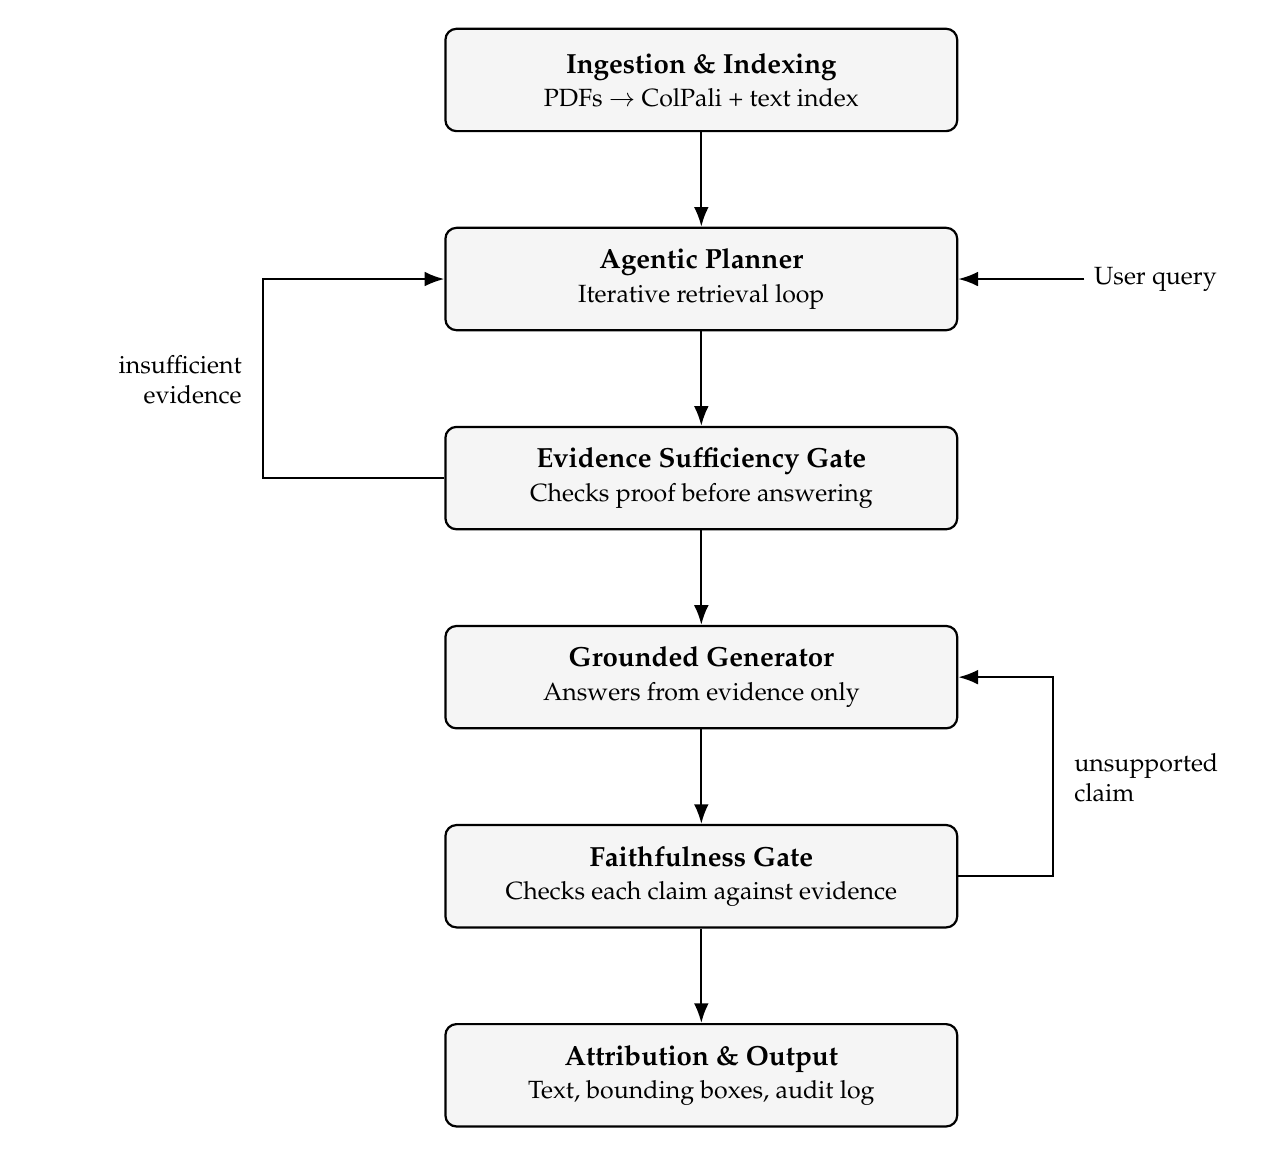
\begin{tikzpicture}[
        node distance=1.2cm and 2.5cm,
        box/.style={rectangle, rounded corners, draw=black, thick, minimum width=6.5cm, minimum height=1.3cm, align=center, fill=gray!8},
        arrow/.style={-{Latex[length=2.5mm]}, thick}
    ]

    \node[box] (ingest) {\textbf{Ingestion \& Indexing} \\ \small PDFs $\rightarrow$ ColPali + text index};
    \node[box, below=of ingest] (planner) {\textbf{Agentic Planner} \\ \small Iterative retrieval loop};
    \node[box, below=of planner] (gate) {\textbf{Evidence Sufficiency Gate} \\ \small Checks proof before answering};
    \node[box, below=of gate] (gen) {\textbf{Grounded Generator} \\ \small Answers from evidence only};
    \node[box, below=of gen] (faith) {\textbf{Faithfulness Gate} \\ \small Checks each claim against evidence};
    \node[box, below=of faith] (answer) {\textbf{Attribution \& Output} \\ \small Text, bounding boxes, audit log};

    \draw[arrow] (ingest) -- (planner);
    \draw[arrow] (planner) -- (gate);
    \draw[arrow] (gate) -- (gen);
    \draw[arrow] (gen) -- (faith);
    \draw[arrow] (faith) -- (answer);

    \node[right=1.6cm of planner] (query) {\small User query};
    \draw[arrow] (query) -- (planner);

    \draw[arrow] (gate.west) -- ++(-2.3,0) coordinate (loopPoint) |- (planner.west);
    \node[anchor=east, font=\small, text width=2.6cm, align=right] at ($(loopPoint) + (-0.15,1.25)$) {insufficient evidence};

    \draw[arrow] (faith.east) -- ++(1.2,0) coordinate (loopPoint2) |- (gen.east);
    \node[anchor=west, font=\small, text width=2.2cm, align=left] at ($(loopPoint2) + (0.15,1.25)$) {unsupported claim};

    \end{tikzpicture}
    \caption{High-level architecture of the multimodal agentic literature review system.}
    \label{fig:architecture}
\end{figure}

\section{Ingestion and Indexing Layer}
Each PDF page in the corpus is rasterized into a page image, which is embedded using a visual document retriever (ColPali~\cite{faysse2025colpali}) to produce patch-level embeddings without requiring OCR or layout parsing. In parallel, narrative text is extracted and segmented into chunks, which are embedded using a retrieval-trained scientific text encoder (SPECTER2~\cite{singh2023scirepeval}) and stored in a FAISS~\cite{johnson2019faiss} index. This produces two complementary indexes:
\begin{itemize}
    \item \textbf{Visual index:} Page-level patch embeddings for retrieving tables, figures, and dense visual content.
    \item \textbf{Textual index:} Chunk-level embeddings for retrieving narrative claims and discussion.
\end{itemize}

\section{Agentic Planner}
The Agentic Planner is an LVLM-driven controller that operates an iterative reasoning loop (Thought $\rightarrow$ Action $\rightarrow$ Observation), inspired by the ReAct paradigm~\cite{yao2023react}. At each step, the planner selects one of the following tools, which correspond to the action space $\mathcal{A}$ defined in Chapter~\ref{sec:methodology}:
\begin{itemize}
    \item \texttt{TextRetriever(query)}: dense retrieval over the textual index.
    \item \texttt{TableRetriever(query)}: locates a table through the visual index, then parses it with a table-structure recogniser~\cite{smock2022pubtables} into structured form, preserving the page coordinates of every cell.
    \item \texttt{FigureRetriever(query)}: visual retrieval over the ColPali index, returning pages together with their patch-similarity scores.
    \item \texttt{RegionZoom(page\_id, bbox)}: crops a sub-region of a retrieved page and re-encodes it at higher resolution for closer inspection of dense tables or charts.
\end{itemize}
Multi-hop navigation (for example, from a textual claim to its supporting table) requires no dedicated tool: it arises from the loop itself, since each retrieved observation informs the query the planner issues next. All tool invocations and their results are recorded in a structured scratchpad, which later serves as the auditable retrieval log referenced in Chapter~\ref{sec:introduction}.

\section{Evidence Sufficiency Gate}
After each retrieval round, the Evidence Sufficiency Gate determines whether the evidence accumulated in the scratchpad is sufficient to answer the query. Two candidate implementations are considered:
\begin{itemize}
    \item \textbf{LLM-as-judge gate:} A prompted model evaluates the query and current evidence, returning a structured judgment of sufficiency and any missing information.
    \item \textbf{Learned gate:} A lightweight classifier trained on retrieval confidence scores and evidence coverage features.
\end{itemize}
If the gate reports insufficient evidence, control returns to the Agentic Planner for an additional retrieval iteration, bounded by a maximum iteration count to prevent unbounded looping. This mechanism directly implements Objective 3 and mitigates hallucination by preventing the system from answering without grounded proof.

\section{Grounded Generator and Faithfulness Gate}
Once the Sufficiency Gate confirms sufficiency, an open-weight vision-language model run locally (such as Qwen2-VL~\cite{wang2024qwen2vl}) generates an answer strictly conditioned on the retrieved evidence pool; the generator has no other access to the corpus. Local weights are required so that token attribution can compute gradients through the generator. The Faithfulness Gate then decomposes the draft into individual claims and checks each against the evidence pool. Any unsupported claim sends the draft back to the generator for rewriting, again bounded by a maximum iteration count.

\section{Attribution Layer}
Visual attribution is produced from two sources preserved during retrieval: the cell coordinates recorded by \texttt{TableRetriever}, and the patch-level similarity scores from the ColPali retrieval step, which localize the most relevant region of a source figure. Together these yield bounding-box coordinates over the supporting table cell or figure region. This satisfies Objective 4 and provides the fine-grained visual grounding required for human verifiability (RQ3).

\section{Mapping to Research Objectives}
Table~\ref{tab:objective-mapping} summarizes how each architectural component addresses the research objectives introduced in Chapter~\ref{sec:introduction}.

\begin{table}[htbp]
    \centering
    \begin{tabular}{ll}
        \toprule
        \textbf{Component} & \textbf{Research Objective} \\
        \midrule
        Ingestion and Indexing Layer & Objective 2 \\
        Agentic Planner & Objective 1 \\
        Evidence Sufficiency Gate & Objective 3 \\
        Grounded Generator and Faithfulness Gate & Objective 3 \\
        Attribution Layer & Objective 4 \\
        \bottomrule
    \end{tabular}
    \caption{Mapping of architectural components to research objectives.}
    \label{tab:objective-mapping}
\end{table}
\chapter{Graph Architecture and Node Specification}
\label{sec:graph}

This chapter describes the system as a graph: a set of nodes, each with one job,
connected by edges that show what flows between them. The goal is that this graph
can be built node-for-node in a framework such as LangGraph~\cite{langgraph}, with nothing left to
guess between what the thesis says and what the code does.

\section{Design Rationale}

Two design choices set this system apart from a standard single-pass RAG pipeline.

\textbf{Retrieval can repeat.} A standard pipeline searches once and answers once,
so it only works if that one search happens to find everything needed. Here, the
planner (N5) can call retrieval tools again and again, and the Sufficiency Gate
sends it back until the evidence is actually enough. Multi-hop reasoning is not a
prompting trick; it is simply how the loop is built.

\textbf{Only certain nodes can add evidence.} Nodes N6a--N7 are the only ones
allowed to bring anything into the evidence buffer (N8), and the generator (N9) can
only read from that buffer --- it has no other way to see the corpus. This
separation is what makes the Faithfulness Gate work: it only has to check claims
against one fixed source of truth, instead of guessing whether the generator made
something up.

\begin{figure}[p]
\centering
\resizebox{!}{0.72\textheight}{%
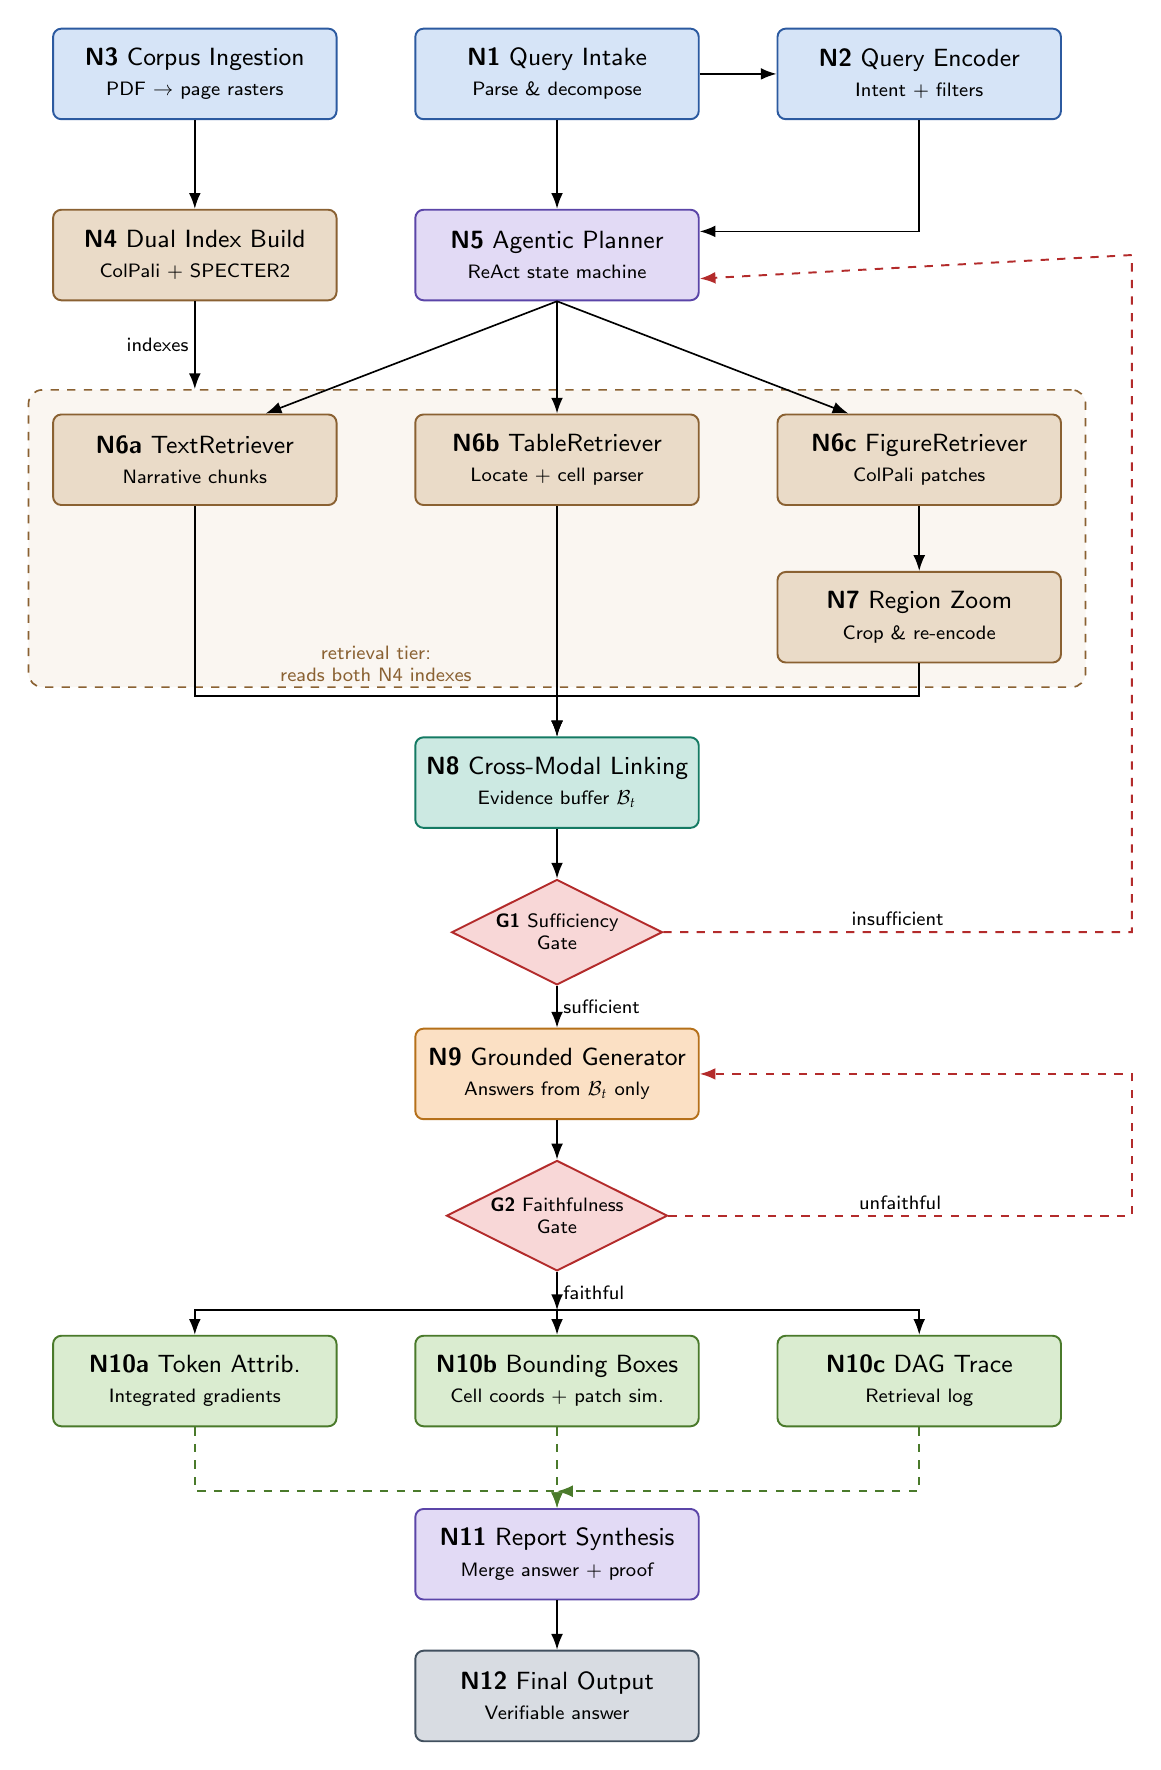
\begin{tikzpicture}[
  font=\sffamily,
  nd/.style={rectangle, rounded corners=3pt, draw, line width=0.7pt, minimum width=3.6cm, minimum height=1.15cm, align=center, inner sep=3pt, font=\sffamily\small},
  enc/.style={nd, fill=encblue, draw=encline},
  ret/.style={nd, fill=retbrown, draw=retline},
  fus/.style={nd, fill=fusteal, draw=fusline},
  svc/.style={nd, fill=svcorange, draw=svcline},
  sup/.style={nd, fill=supviolet, draw=supline},
  att/.style={nd, fill=attgreen, draw=attline},
  fin/.style={nd, fill=darkslate, draw=darkline},
  gate/.style={diamond, aspect=2.0, draw=gateline, line width=0.7pt, fill=gatered, align=center, inner sep=1pt, font=\sffamily\scriptsize},
  ar/.style={-{Latex[length=2mm]}, line width=0.6pt},
  loop/.style={-{Latex[length=2mm]}, line width=0.7pt, draw=gateline, dashed},
  back/.style={-{Latex[length=2mm]}, line width=0.6pt, draw=attline, dashed},
  lbl/.style={font=\sffamily\scriptsize, inner sep=2pt}
]

\node[enc] (n3) at (-4.6,0)    {\textbf{N3} Corpus Ingestion\\\scriptsize PDF $\rightarrow$ page rasters};
\node[enc] (n1) at (0,0)       {\textbf{N1} Query Intake\\\scriptsize Parse \& decompose};
\node[enc] (n2) at (4.6,0)     {\textbf{N2} Query Encoder\\\scriptsize Intent + filters};

\node[ret] (n4) at (-4.6,-2.3) {\textbf{N4} Dual Index Build\\\scriptsize ColPali + SPECTER2};
\node[sup] (n5) at (0,-2.3)    {\textbf{N5} Agentic Planner\\\scriptsize ReAct state machine};

\node[ret] (n6a) at (-4.6,-4.9){\textbf{N6a} TextRetriever\\\scriptsize Narrative chunks};
\node[ret] (n6b) at (0,-4.9)   {\textbf{N6b} TableRetriever\\\scriptsize Locate + cell parser};
\node[ret] (n6c) at (4.6,-4.9) {\textbf{N6c} FigureRetriever\\\scriptsize ColPali patches};

\node[ret] (n7) at (4.6,-6.9)  {\textbf{N7} Region Zoom\\\scriptsize Crop \& re-encode};

\node[fus] (n8) at (0,-9.0)    {\textbf{N8} Cross-Modal Linking\\\scriptsize Evidence buffer $\mathcal{B}_t$};

\node[gate] (g1) at (0,-10.9)  {\textbf{G1} Sufficiency\\Gate};

\node[svc] (n9) at (0,-12.7)   {\textbf{N9} Grounded Generator\\\scriptsize Answers from $\mathcal{B}_t$ only};

\node[gate] (g2) at (0,-14.5)  {\textbf{G2} Faithfulness\\Gate};

\node[att] (n10a) at (-4.6,-16.6){\textbf{N10a} Token Attrib.\\\scriptsize Integrated gradients};
\node[att] (n10b) at (0,-16.6)   {\textbf{N10b} Bounding Boxes\\\scriptsize Cell coords + patch sim.};
\node[att] (n10c) at (4.6,-16.6) {\textbf{N10c} DAG Trace\\\scriptsize Retrieval log};

\node[sup] (n11) at (0,-18.8)  {\textbf{N11} Report Synthesis\\\scriptsize Merge answer + proof};
\node[fin] (n12) at (0,-20.6)  {\textbf{N12} Final Output\\\scriptsize Verifiable answer};

\draw[ar] (n1) -- (n2);
\draw[ar] (n1) -- (n5);
\draw[ar] (n2.south) |- ([yshift=0.3cm]n5.east);
\draw[ar] (n3) -- (n4);

\begin{scope}[on background layer]
  \node[draw=retline, dashed, rounded corners=5pt, line width=0.6pt, fill=retbrown!25,
        fit=(n6a)(n6b)(n6c)(n7), inner sep=0.3cm] (tier) {};
\end{scope}
\node[lbl, anchor=south, text=retline, align=center] at (-2.3,0 |- tier.south) {retrieval tier:\\reads both N4 indexes};
\draw[ar] (n4.south) -- (n4.south |- tier.north) node[lbl, midway, left]{indexes};

\draw[ar] (n5.south) -- ([xshift=0.9cm]n6a.north);
\draw[ar] (n5) -- (n6b);
\draw[ar] (n5.south) -- ([xshift=-0.9cm]n6c.north);
\draw[ar] (n6c) -- (n7);

\draw[ar] (n6a.south) -- (-4.6,-7.9) -| (n8.north);
\draw[ar] (n7.south) -- (4.6,-7.9) -| (n8.north);
\draw[ar] (n6b) -- (n8);

\draw[ar] (n8) -- (g1);
\draw[ar] (g1) -- node[lbl, midway, right]{sufficient} (n9);
\draw[ar] (n9) -- (g2);

\draw[loop] (g1.east) -- node[lbl, pos=0.5, above, black]{insufficient} (7.3,-10.9) -- (7.3,-2.3) -- ([yshift=-0.3cm]n5.east);
\draw[loop] (g2.east) -- node[lbl, pos=0.5, above, black]{unfaithful} (7.3,-14.5) -- (7.3,-12.7) -- (n9.east);

\draw[ar] (g2.south) -- node[lbl, pos=0.55, right]{faithful} (0,-15.7);
\draw[ar] (0,-15.7) -- (-4.6,-15.7) -- (n10a.north);
\draw[ar] (0,-15.7) -- (4.6,-15.7) -- (n10c.north);
\draw[ar] (0,-15.7) -- (n10b.north);

\draw[back] (n10a.south) -- (-4.6,-18.0) -- (0,-18.0) -- (n11.north);
\draw[back] (n10c.south) -- (4.6,-18.0) -- (0,-18.0);
\draw[back] (n10b) -- (n11);
\draw[ar] (n11) -- (n12);

\end{tikzpicture}%
}
\caption{Full graph architecture of the proposed Agentic Multimodal RAG system.
Blue nodes perform ingestion and query encoding; brown nodes are the retrieval
tools that hold exclusive authority to introduce evidence, grouped in the shaded
retrieval tier because all of them query the two indexes built by N4; the teal node maintains
the evidence buffer that every downstream node reads from; the orange node is the
grounded generator; violet nodes are the planner and the synthesiser; green nodes
produce the three attribution artefacts. Red diamonds are the two validation gates
and red dashed edges are the two correction loops. Green dashed edges carry
attribution artefacts forward to synthesis. The planner may traverse the retrieval
tier arbitrarily many times before the Sufficiency Gate permits generation.}
\label{fig:graph}
\end{figure}

\section{Node-by-Node Specification}

Here is how one query moves through the graph, start to finish.

\begin{quote}
\textbf{Running example.} \emph{``Does the reported accuracy gain in Section~4 hold
for the low-resource subset, and which table reports it?''}
\end{quote}

This question needs two different kinds of evidence: a claim from the text and a
number from a table. A single search cannot answer it alone, which is exactly why
it is used here.

\subsection{Ingestion Path (N3--N4)}

This part runs once per corpus, offline, before any query arrives.

\paragraph{N3 --- Corpus Ingestion.}
Every PDF page is converted into an image, and its text is separately pulled out
and split into chunks. Pages become images rather than parsed layouts because
tables are exactly where OCR fails --- merged cells and multi-column headers break
text extraction. An image keeps the table's structure intact.

\paragraph{N4 --- Dual Index Build.}
Two search indexes are built from the same set of pages: one holds ColPali
visual embeddings of each page image (for finding tables and figures), the other
holds SPECTER2 text embeddings of each chunk, stored in FAISS~\cite{johnson2019faiss}
(for finding claims). Every retrieval tool (N6a--N6c, N7) reads from these two
indexes. Because both indexes point back
to the same pages, a match in one can lead directly to the matching spot in the
other --- which is what makes jumping from a text claim to its supporting table
possible.

\subsection{Query Encoding Path (N1--N2)}

\paragraph{N1 --- Query Intake.}
The question is broken into smaller steps before any search happens. For the
running example, that is two steps: find the accuracy claim, then find the table
that reports the low-resource breakdown. Doing this upfront gives the planner a
plan to follow instead of improvising one.

\paragraph{N2 --- Query Encoder.}
The query is embedded, and filters are pulled out of it --- here, ``Section 4'' and
``low-resource subset.'' This has to finish before any retrieval starts, since
every search the planner runs afterward depends on these filters.

\subsection{Planning and Retrieval (N5--N7)}

\paragraph{N5 --- Agentic Planner.}
This is the only node that decides what happens next. It keeps track of the plan,
what has already been searched, and what evidence has been found, then picks one
retrieval tool to run. After seeing the result, it either searches again or moves
on to the Sufficiency Gate. It never adds evidence itself --- only a retrieval tool
can do that.

\paragraph{N6a --- TextRetriever.}
Searches the text index for narrative chunks matching the query. On the running
example, this is the first search: it finds the sentence claiming the accuracy
gain, along with the page it appears on.

\paragraph{N6b --- TableRetriever.}
Finds a table in two steps: it searches the visual index for pages whose best
match is a table, then runs a table-structure recogniser (such as the Table
Transformer) on that region to recover rows, columns and the position of every
cell. Cell text is read from the PDF at those positions. It keeps track of exactly
where each cell sits on the page. This matters because the bounding boxes generated later (N10b) are only
possible if this spatial position is kept --- a plain-text version of the table
would lose it.

\paragraph{N6c --- FigureRetriever (ColPali).}
Searches the visual index to find charts, plots, or dense tables without needing
OCR. It also keeps the match scores it computed, because those scores are reused
later to draw bounding boxes.

\paragraph{N7 --- Region Zoom.}
Crops in on part of a page and re-encodes it at higher resolution. This exists
because finding the right page and reading a specific row inside it need different
levels of detail --- a page-level match tells you which page has the table, not
which row answers the question. On the running example, this runs after N6c finds
the right page, zooming into the low-resource row so its cells become readable.

\subsection{Evidence Buffer and Sufficiency Gate (N8, G1)}

\paragraph{N8 --- Cross-Modal Linking.}
Everything retrieved so far is converted into one shared format and added to the
evidence buffer, along with where it came from --- which page, which tool, which
step. Items that share a page, or where one refers to the other (a sentence citing
``Table~3'' and the table captioned ``Table~3''), are linked, so that the generator
receives connected evidence rather than a loose pile. This buffer is the only thing the generator will ever see; nothing after this
point looks at the corpus again.

\paragraph{G1 --- Sufficiency Gate.}
Before generation is allowed, a check runs: is there enough evidence here to
actually answer the question? On the running example, the first check fails --- the
text claim is there, but the table that would confirm or deny it for the
low-resource subset is not. Control goes back to N5, which fetches the table. Only
once both pieces are present does the gate let the process continue.

This check happens \emph{before} generation, not after. A standard pipeline would
hand the incomplete evidence to the generator and hope it notices something is
missing --- which is exactly how confident, wrong answers get produced.

\subsection{Generation and Faithfulness Gate (N9, G2)}

\paragraph{N9 --- Grounded Generator.}
An open-weight vision-language model (such as Qwen2-VL) run locally, so that N10a
can compute gradients through it. It writes the answer using only what is in the
evidence buffer. It cannot search on
its own and cannot fill in numbers from memory --- everything it says has to trace
back to something already retrieved.

\paragraph{G2 --- Faithfulness Gate.}
Checks every factual claim in the draft answer against the evidence buffer. If the
answer states something that is not actually backed by retrieved evidence, the
gate fails and N9 is sent back to rewrite that part using only what is really
there. Because the buffer is the only source allowed, each claim is checked
against one fixed, finite list of retrieved items, rather than against everything
the model might believe about the world.

\subsection{Attribution and Output (N10--N12)}

\paragraph{N10a --- Token Attribution.}
Highlights which retrieved sentences most influenced each part of the answer, using
integrated gradients computed through the N9 generator.

\paragraph{N10b --- Bounding Boxes.}
Draws a box --- $[x_{\min}, y_{\min}, x_{\max}, y_{\max}]$ --- around the exact spot
on the page a claim came from. For a table cell, the box is the cell position N6b
recorded; for a figure, it encloses the highest-scoring patches from N6c (or N7).
This only works because N6b kept cell positions and N6c kept its match scores.

\paragraph{N10c --- DAG Trace.}
Logs what actually happened: which tools ran, in what order, and how many times the
Sufficiency Gate sent things back. On the running example, this log shows two
search rounds and one rejection --- so the process can be checked, not just
trusted.

\paragraph{N11 --- Report Synthesis.}
Combines the answer with its three proof artefacts into one readable report.

\paragraph{N12 --- Final Output.}
What the user actually sees: the answer, the highlighted source text, a box on the
source page, and the log of how it was found.

\section{Control Loops}

There are exactly two loops in this graph, and each catches a different kind of
mistake.

\paragraph{The retrieval loop (not enough evidence).}
Triggered by the Sufficiency Gate. Sends control back to N5 to search again. This
stops the system from confidently answering using incomplete evidence.

\paragraph{The regenerate loop (wrong evidence used).}
Triggered by the Faithfulness Gate. Sends control back to N9 to rewrite. This stops
the system from stating something the evidence does not actually support.

Both loops have a limit on how many times they can repeat. If that limit is
reached, the system says the evidence is not enough instead of guessing. For a
literature review tool, this is the right trade-off: ``I could not confirm this''
is useful. A confident wrong answer is not.

\section{Mapping to Research Objectives}

Table~\ref{tab:node-mapping} shows which objective each part of the graph is
responsible for.

\begin{table}[htbp]
\centering
\small
\begin{tabular}{llp{5.4cm}}
\toprule
\textbf{Nodes} & \textbf{Objective} & \textbf{Contribution} \\
\midrule
N3, N4, N6c & Objective 2 & Vision-document retrieval over rasterised pages \\
N1, N2, N5, N7 & Objective 1 & Iterative agentic planning and multi-hop navigation \\
N8, Sufficiency Gate & Objective 3 & Evidence verification prior to generation \\
N9, Faithfulness Gate & Objective 3 & Claim-level grounding of generated output \\
N10a--N10c, N11 & Objective 4 & Spatial, textual, and procedural attribution \\
\bottomrule
\end{tabular}
\caption{Mapping of graph nodes to research objectives.}
\label{tab:node-mapping}
\end{table}

% --- References ---
\cleardoublepage
\phantomsection
\addcontentsline{toc}{chapter}{Bibliography}
\bibliographystyle{plain}
\bibliography{references}

\end{document}